\documentclass[border=4pt,12pt]{standalone}
% House style for redrawn exam diagrams (diagram-v4: 0.4pt lines, filled -latex arrows, fine dashes; stipple and hatching drawn as real dots/lines (no PDF/SVG patterns, so they render in every browser and at any scale); transparent background). Every figure \input's this.
\usepackage{amsmath,amssymb}
\usepackage{txfonts}
\usepackage{pdfrender,xcolor}
% \halo{text}: label on shading. The shading stops just around each letter's outline (a thin knock-out that follows the
% glyphs, like the papers' typesetting), never a box. Owner: "I don't want a box around the text".
\newcommand{\halo}[1]{\leavevmode\rlap{\pdfrender{TextRenderingMode=2,LineWidth=2.2pt,LineJoinStyle=1,StrokeColor=white,FillColor=white}#1}#1}
\usepackage{tikz,pgfplots}
\pgfplotsset{compat=1.18}
\usetikzlibrary{arrows.meta,calc,angles,quotes,patterns,patterns.meta,intersections,positioning,decorations.markings,shapes.geometric}
% Stipple and hatching are drawn as actual dots / lines clipped to the region (path picture), NOT as pattern fills:
% SVG <pattern> fills vanish or blur when browsers scale the image, so the owner could not see the shading.
% Each dot is a 0.72pt square (keeps SVGs small; reads as a dot at print size). Dots sit on one global staggered grid, so neighbouring regions line up.
\makeatletter
\newdimen\ex@x \newdimen\ex@y \newdimen\ex@xa \newdimen\ex@ya \newdimen\ex@xb \newdimen\ex@yb \newcount\ex@row
\def\exam@stipplecolor{black!75}\def\exam@dotr{0.42pt}\def\exam@dotgap{2.5}
\def\ex@rowdots{\ifdim\ex@x<\ex@xb \pgfpathrectangle{\pgfqpoint{\dimexpr\ex@x-0.36pt\relax}{\dimexpr\ex@y-0.36pt\relax}}{\pgfqpoint{0.72pt}{0.72pt}}\advance\ex@x by \exam@dotgap pt\relax\expandafter\ex@rowdots\fi}
\def\exam@stipple{%
  \pgftransformreset% dots are sized in real points even inside scaled pictures
  \pgfpointanchor{path picture bounding box}{south west}\ex@xa=\pgf@x \ex@ya=\pgf@y
  \pgfpointanchor{path picture bounding box}{north east}\ex@xb=\pgf@x \ex@yb=\pgf@y
  \pgfsetfillcolor{\exam@stipplecolor}\pgfmathsetmacro\ex@h{\exam@dotgap/2}%
  \pgfmathtruncatemacro\ex@r{floor(\ex@ya/\ex@h)-1}\ex@row=\ex@r\relax
  \ex@y=\ex@r\dimexpr\ex@h pt\relax
  \loop\ifdim\ex@y<\ex@yb
    \pgfmathtruncatemacro\ex@c{floor(\ex@xa/\exam@dotgap)-1}\ex@x=\ex@c\dimexpr\exam@dotgap pt\relax
    \ifodd\ex@row \advance\ex@x by \ex@h pt\fi
    \ex@rowdots
    \advance\ex@y by \ex@h pt \advance\ex@row by 1
    \ifnum\numexpr\ex@row-(\ex@row/4)*4\relax=0 \pgfusepath{fill}\fi% flush every 4 rows: bounded TeX memory, few clip copies in the SVG
  \repeat\pgfusepath{fill}}
\newdimen\ex@d
\def\exam@hatch#1{% #1 = 1 for /, -1 for \ ; lines 45 degrees, 3pt apart
  \pgftransformreset
  \pgfpointanchor{path picture bounding box}{south west}\ex@xa=\pgf@x \ex@ya=\pgf@y
  \pgfpointanchor{path picture bounding box}{north east}\ex@xb=\pgf@x \ex@yb=\pgf@y
  \ex@d=\dimexpr\ex@yb-\ex@ya\relax \ex@x=\dimexpr\ex@xa-\ex@d\relax
  \loop\ifdim\ex@x<\ex@xb
    \ifnum#1>0 \pgfpathmoveto{\pgfqpoint{\ex@x}{\ex@ya}}\pgfpathlineto{\pgfqpoint{\dimexpr\ex@x+\ex@d\relax}{\ex@yb}}%
    \else \pgfpathmoveto{\pgfqpoint{\ex@x}{\ex@yb}}\pgfpathlineto{\pgfqpoint{\dimexpr\ex@x+\ex@d\relax}{\ex@ya}}\fi
    \advance\ex@x by 4.24pt
  \repeat
  \pgfsetlinewidth{0.4pt}\pgfsetstrokecolor{black}\pgfusepath{stroke}}
\def\examstipple{\exam@stipple}\def\examhatch{\exam@hatch}\def\examsetstipplecolor#1{\def\exam@stipplecolor{#1}}\def\examsetdotgap#1{\def\exam@dotgap{#1}}
\makeatother
% (legacy pattern kept for old files)
% staggered stipple like the NESA papers' dotted shading
\pgfdeclarepatternformonly{exam stipple}{\pgfpointorigin}{\pgfqpoint{2.2pt}{2.2pt}}{\pgfqpoint{2.2pt}{2.2pt}}{%
  \pgfpathcircle{\pgfqpoint{0.55pt}{0.55pt}}{0.42pt}\pgfpathcircle{\pgfqpoint{1.65pt}{1.65pt}}{0.42pt}\pgfusepath{fill}}
\tikzset{
  every picture/.style={line width=0.6pt, >={Latex[length=2mm,width=1.3mm]}},
  curve/.style={line width=0.6pt},
  open arrow/.style={-{Latex[length=2mm,width=1.3mm]}},  % owner: filled -latex heads everywhere, no open chevrons
  aux/.style={dash pattern=on 2pt off 1.5pt, line width=0.6pt},
  shade/.code={\def\exA{#1}\def\exB{none}\ifx\exA\exB\else\pgfkeysalso{fill=black!18}\fi},
  shade/.default=on,
  shade dots/.style={fill=none, path picture={\examstipple}},
  stipple color/.code={\examsetstipplecolor{#1}},
  stipple gap/.code={\examsetdotgap{#1}},
  shade dense dots/.style={fill=none, stipple gap=1.6, path picture={\examstipple}},
  shade hatch/.style={fill=none, path picture={\examhatch{1}}},
  shade hatch reverse/.style={fill=none, path picture={\examhatch{-1}}},
  shade solid/.style={fill=black},
  pt/.style={circle, fill, inner sep=1.1pt},
  open pt/.style={circle, draw, fill=white, inner sep=1.1pt},
}
\pgfplotsset{
  exam axes/.style={axis lines=middle, axis line style={->}, xlabel={$x$}, ylabel={$y$},
    xlabel style={anchor=west}, ylabel style={anchor=south}, tick label style={font=\small},
    every axis plot/.append style={line width=0.6pt, black}, samples=200, clip=false,
    enlargelimits=false, axis on top},
}

\begin{document}
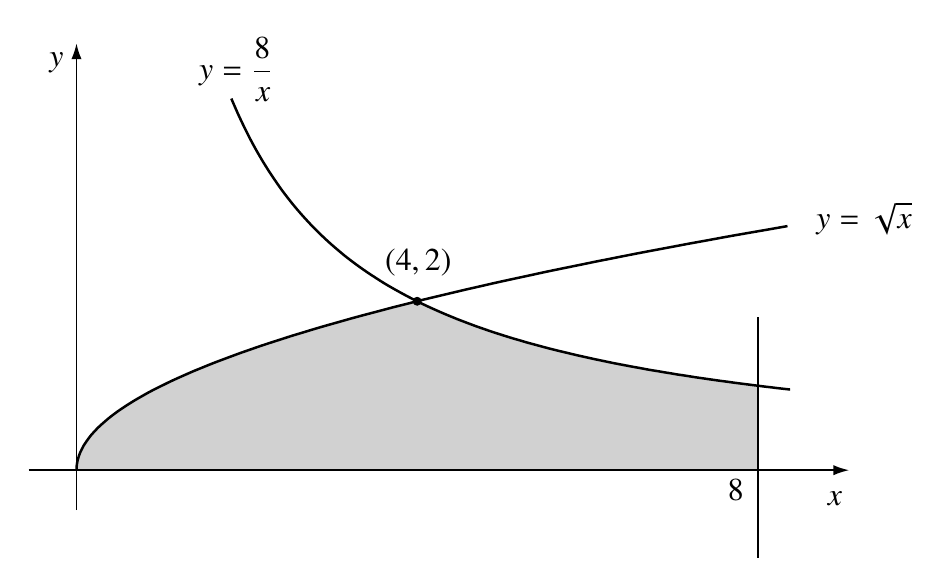
\begin{tikzpicture}[x=0.0127cm,y=-0.0127cm,font=\fontsize{11.5}{13.799999999999999}\selectfont]
\fill[shade] plot[smooth] coordinates {(78.0,490.0) (78.1,486.6) (78.6,483.1) (79.3,479.7) (80.3,476.2) (81.5,472.8) (83.1,469.3) (85.0,465.9) (87.1,462.4) (89.5,459.0) (92.2,455.5) (95.2,452.1) (98.4,448.6) (102.0,445.2) (105.8,441.7) (109.9,438.3) (114.3,434.8) (119.0,431.4) (124.0,427.9) (129.2,424.5) (134.8,421.0) (140.6,417.6) (146.7,414.1) (153.1,410.7) (159.7,407.2) (166.7,403.8) (173.9,400.3) (181.5,396.9) (189.3,393.4) (197.4,390.0) (205.7,386.5) (214.4,383.1) (223.3,379.6) (232.6,376.2) (242.1,372.7) (251.9,369.3) (261.9,365.8) (272.3,362.4) (282.9,358.9) (293.9,355.5) (305.1,352.0) (316.6,348.6) (328.4,345.1) (340.4,341.7) (352.8,338.2) (365.4,334.8) (378.3,331.3) (391.5,327.9) (405.0,324.4) (418.8,321.0)} -- plot[smooth] coordinates {(418.8,321.0) (430.5,326.6) (442.3,331.9) (454.0,336.8) (465.8,341.5) (477.5,345.9) (489.3,350.0) (501.0,353.9) (512.8,357.5) (524.5,361.0) (536.3,364.3) (548.0,367.5) (559.8,370.5) (571.5,373.3) (583.3,376.0) (595.0,378.6) (606.8,381.1) (618.5,383.5) (630.3,385.7) (642.0,387.9) (653.8,390.0) (665.5,392.0) (677.3,393.9) (689.0,395.8) (700.8,397.5) (712.5,399.2) (724.3,400.9) (736.0,402.5) (747.8,404.0) (759.5,405.5)} -- (759.5,490) -- cycle;
\draw[->] (30,490)--(851,490); \draw[->] (78,530)--(78,63);
\draw (759.5,337)--(759.5,578);
\draw[line width=0.9pt] plot[smooth] coordinates {(78.0,490.0) (78.1,486.5) (78.6,482.9) (79.3,479.4) (80.4,475.8) (81.7,472.3) (83.4,468.8) (85.3,465.2) (87.6,461.7) (90.1,458.2) (92.9,454.6) (96.1,451.1) (99.5,447.5) (103.3,444.0) (107.3,440.5) (111.6,436.9) (116.2,433.4) (121.2,429.8) (126.4,426.3) (131.9,422.8) (137.8,419.2) (143.9,415.7) (150.3,412.1) (157.0,408.6) (164.1,405.1) (171.4,401.5) (179.0,398.0) (186.9,394.5) (195.1,390.9) (203.7,387.4) (212.5,383.8) (221.6,380.3) (231.0,376.8) (240.7,373.2) (250.7,369.7) (261.0,366.1) (271.6,362.6) (282.5,359.1) (293.7,355.5) (305.3,352.0) (317.1,348.4) (329.2,344.9) (341.6,341.4) (354.3,337.8) (367.3,334.3) (380.6,330.8) (394.1,327.2) (408.0,323.7) (422.2,320.1) (436.7,316.6) (451.5,313.1) (466.6,309.5) (482.0,306.0) (497.7,302.4) (513.7,298.9) (530.0,295.4) (546.5,291.8) (563.4,288.3) (580.6,284.8) (598.1,281.2) (615.9,277.7) (634.0,274.1) (652.3,270.6) (671.0,267.1) (690.0,263.5) (709.3,260.0) (728.8,256.4) (748.7,252.9) (768.9,249.4) (789.3,245.8)};
\draw[line width=0.9pt] plot[smooth] coordinates {(232.9,118.2) (239.2,132.7) (245.5,146.1) (251.7,158.5) (258.0,170.1) (264.3,180.9) (270.6,191.0) (276.9,200.4) (283.1,209.3) (289.4,217.6) (295.7,225.5) (302.0,232.9) (308.3,239.9) (314.5,246.5) (320.8,252.8) (327.1,258.8) (333.4,264.5) (339.7,269.9) (345.9,275.1) (352.2,280.0) (358.5,284.7) (364.8,289.2) (371.1,293.5) (377.4,297.6) (383.6,301.6) (389.9,305.4) (396.2,309.0) (402.5,312.5) (408.8,315.9) (415.0,319.1) (421.3,322.3) (427.6,325.3) (433.9,328.2) (440.2,331.0) (446.4,333.7) (452.7,336.3) (459.0,338.9) (465.3,341.3) (471.6,343.7) (477.8,346.0) (484.1,348.2) (490.4,350.4) (496.7,352.5) (503.0,354.5) (509.3,356.5) (515.5,358.4) (521.8,360.2) (528.1,362.1) (534.4,363.8) (540.7,365.5) (546.9,367.2) (553.2,368.8) (559.5,370.4) (565.8,371.9) (572.1,373.4) (578.3,374.9) (584.6,376.3) (590.9,377.7) (597.2,379.1) (603.5,380.4) (609.7,381.7) (616.0,383.0) (622.3,384.2) (628.6,385.4) (634.9,386.6) (641.2,387.7) (647.4,388.9) (653.7,390.0) (660.0,391.0) (666.3,392.1) (672.6,393.1) (678.8,394.2) (685.1,395.1) (691.4,396.1) (697.7,397.1) (704.0,398.0) (710.2,398.9) (716.5,399.8) (722.8,400.7) (729.1,401.5) (735.4,402.4) (741.6,403.2) (747.9,404.0) (754.2,404.8) (760.5,405.6) (766.8,406.4) (773.0,407.1) (779.3,407.9) (785.6,408.6) (791.9,409.3)};
\fill (418.8,321.0) circle (4.5);
\node at (58,82) {$y$}; \node at (836,518) {$x$}; \node at (737.5,510) {$8$}; \node at (420,282) {$(4,2)$};
\node at (238,89) {$y=\dfrac{8}{x}$}; \node at (866,238) {$y=\sqrt{x}$};\end{tikzpicture}
\end{document}
